
% Begin with describing virtual circuit switching
\begin{section}{Virtual Circuit Switching}

Virtual Circuit Switching is a method of switching in which a dedicated path is established between the source and destination before the actual data transfer begins. This path is called a virtual circuit. The virtual circuit is a logical path that is established between the source and destination. The virtual circuit is established by sending a setup message from the source to the destination. The destination sends back an acknowledgment message to the source. Once the virtual circuit is established, the data transfer begins. The data transfer takes place over the virtual circuit. The virtual circuit is torn down after the data transfer is complete. Virtual Circuit Switching is used in ATM (Asynchronous Transfer Mode) networks.

\end{section}


\begin{section}{Experiment}

    To compare the probability of admission of a connection in a virtual circuit switched network in two different topologies under different traffic loads, constraints (pessimistic and optimistic), and routing metrics.

\end{section}

\begin{section}{Variables of the Experiment}

    \begin{subsection}{Topology}
        Two topologies are considered for the experiment:
        \begin{enumerate}
            \item NFSNET Topology : A network with 12 nodes and 15 links.
            \item ARPANET Topology : A network with 20 nodes and 32 links.
        \end{enumerate}
    \end{subsection}

    \begin{subsection}{Connections}
    Two types of connections are possible:
    \begin{enumerate}
        \item Connections between any two nodes chosen uniformly at random. In this case the connections can be denied for two reasons:
        \begin{enumerate}
            \item There is no path between the two nodes.
            \item There is insufficient bandwidth available on the path between the two nodes.
        \end{enumerate}
        \item Connections are chosen randomly from the set of reachable pairs of nodes. In this case the connections can be denied only if bandwidth is insufficient.
    \end{enumerate}
    Since we are only interested in the probability of admission and not the restrictions of the topology, we will consider the second type of connections.
    \end{subsection}

    \begin{subsection}{Traffic Load}
        \begin{enumerate}
            \item Constant traffic load at 64 kbps. This specific value is chosen because voice calls are typically 64 kbps.
            \item Bursty traffic of $(\text{min}, \text{avg}, \text{max}) = (1, x, 10x)$ kbps. The value of $x$ is varied from 2 to 20 with steps of 2.
        \end{enumerate}
    \end{subsection}
    

    \begin{subsection}{Constraints}
        Two types of constraints are considered for the experiment:
        \begin{enumerate}
            \item \textit{Pessimistic constraints}: Assumes each connection uses its maximum bandwidth.
            \item \textit{Optimistic constraints}: Assumes each connections uses bandwidth equal to \\ $\min\left(B_{max},\ B_{avg} + 0.35 \cdot (B_{max} - B_{min}) \right)$
        \end{enumerate}
    \end{subsection}

    \begin{subsection}{Routing Algortithm}
        Two types of routing metrics are considered for computing the shortest and second shortest path: (1) Hop count and (2) Propagation Delay.
    \end{subsection}

\end{section}

\begin{section}{Results}

It was observed that the admission probability is the same for both the routing metrics, Hop count and Propagation Delay. The following plots and observations hold for both these metrics. \\

\begin{figure}[H]
    \centering
    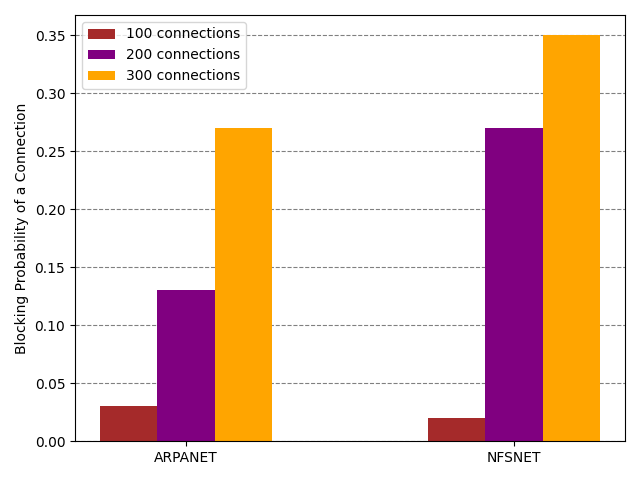
\includegraphics[width=0.8\textwidth]{figures/fig1/fig1.png}
    \caption{Admission Probability with Constant 64kbps Traffic Load \protect\footnotemark}
    \label{fig:fig1}
\end{figure}
\footnotetext{Since the traffic is constant, both optimistic and pessimistic constraints give the same results.}

As is expected, we see that the admission probability decreases as the number of connections increase. This is because the links start getting saturated and available bandwidth becomes insufficient. \\
Also, since the ARPANET topology has more nodes and links than NFSNET, the number of connections needed to saturate most of the links in ARPANET is higher than that for NFSNET. Thus, we see that for the same number of connections, ARPANET has a higher admission probability. \\ 


\pagebreak


\end{section}
